\documentclass[compress,11pt]{beamer}
%\includeonly{pendel}
\usetheme{Ilmenau}
%\usetheme{fau-4-3}
%\usecolortheme{beaver}
\beamertemplatenavigationsymbolsempty
\usepackage[ngerman]{babel}
\usepackage{marvosym}
\usepackage{multimedia}
\usepackage[utf8]{inputenc}
\usepackage{amsmath}
\usepackage{amsfonts}
\usepackage{amssymb}
\usepackage{graphicx}
\usepackage{esvect}
%\author{}
\title{EP Gruppe 8}
%\setbeamercovered{transparent}
%\setbeamertemplate{navigation symbols}{}
%\logo{}
%\institute{}
%\date{}
%\subject{}
\usepackage{verbatim}
\begin{document}


\begin{frame}

\end{frame}

\section{Aufgabe 1: Komparator}
\begin{frame}
Aufzubauen war folgende Schaltung:
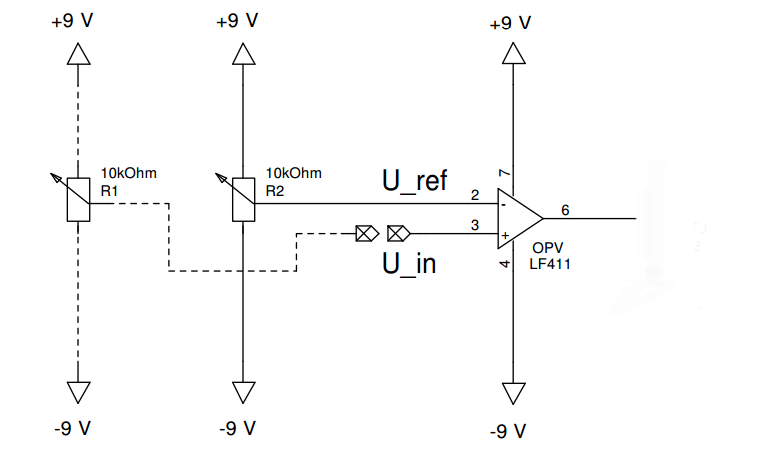
\includegraphics[width=.7\textwidth]{schalt/schalt11}
\end{frame}

\begin{frame}Verwenderter Operationsverstärker
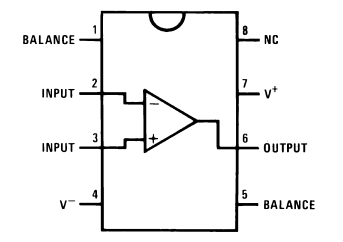
\includegraphics[width=.7\textwidth]{schalt/opamp_innen}
\end{frame}

\begin{frame}
\begin{block}{Zuerst: Funktionsweise des Operationsverstärkers}
\begin{itemize}
\item unser Modell besitzt insgesamt 5 Eingänge; 2 Eingangsspannungs- 1 Ausgangsspannungs- und 2 Versorgungsspannungs-Kontakte
\item verstärkt Differenz der Eingangs-Spannungen $U_{Pin3} - U_{Pin2}$ und gibt diese am Pin 6 aus
\item im Idealfall gilt: Verstärkung $V \rightarrow \infty$
\item $U_{out,min,max}$ ist das positive/negative der Versorgungsspannung (liegt bei unseren Modell an den Pins 4 und 7)
\end{itemize}

\end{block}
\end{frame}

\begin{frame}
Dadurch erklärt sich auch die Komparator-Schaltung:
\begin{itemize}
\item Potentiometer regeln durch ihren variablen Widerstand die Spannung, die an ihnen abfällt
\item durch Variieren der Potentiometer kann nun als Ausgangsspannung die betragsmäßig verringerte minimale oder maximale Versorgungsspannung ausgegeben werden (Verringerung begründet sich durch nicht verschwindende Ausgangsimpedanz)
\end{itemize}
\end{frame}
\begin{frame}
%\includegraphics[scale=•]{•}
Ausgangsspannung über der Differenz der Eingangsspannungen\\ 
Es werden beim "Umschaltpunkt" $U_{diff} = 0$ auch Messwerte zwischen $U_{min}$ und $U_{max}$ gemessen $\Rightarrow$ reale Verstärkung $V < \infty$
\end{frame} 
\begin{frame}
Grobe Abschätzug der Verstärkung:\begin{itemize}

\item Lege eine Steigungsgerade durch den Streifen, in dem zu einem x-Wert verschiedene y-Werte zwischen $U_{min}$ und $U_{max}$ liegen
\item berechne beispielsweise den Mittelwert der $U_{out}$ für $U_{diff} > 0$ und $ < 0$
\item suche die x-Punkte $U_{diff}$, für die sich $U_{out}$ (falls mehrere Messpunkte existieren) nicht mehr wesentlich ändert
\item berechne Differenzenquotient (Die Verstärkung muss mindestens diesem Wert entsprechen)
\end{itemize}
\end{frame}


\begin{frame}
Die Schaltung wurde nun verändert:\\

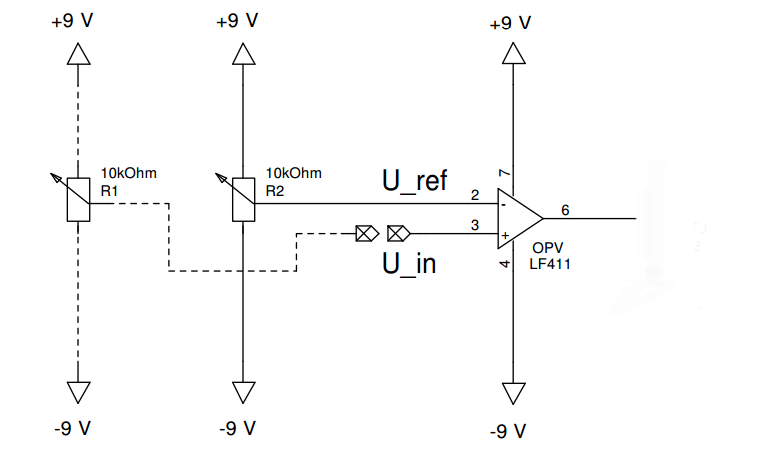
\includegraphics[width=.7\textwidth]{schalt/schalt11}


\end{frame}
\begin{frame}

\end{frame}
\end{document}